\documentclass[aspectratio=169]{beamer}
\useoutertheme[progressbar=frametitle]{metropolis}
\useinnertheme{metropolis}
\definecolor{nabgray}{rgb}{0.6,0.59,0.61}
\usecolortheme[named=nabgray]{structure}


\usepackage{tikz}
\usepackage[utf8]{inputenc}
\usepackage[spanish]{babel}

\usepackage{smartdiagram}
\usepackage{verbatim}
\usepackage{svg}
\usepackage{graphicx}
\usepackage{color}
\definecolor{lightgray}{rgb}{0.95, 0.95, 0.95}
\definecolor{darkgray}{rgb}{0.4, 0.4, 0.4}
%\definecolor{purple}{rgb}{0.65, 0.12, 0.82}
\definecolor{editorGray}{rgb}{0.95, 0.95, 0.95}
\definecolor{editorOcher}{rgb}{1, 0.5, 0} % #FF7F00 -> rgb(239, 169, 0)
\definecolor{editorGreen}{rgb}{0, 0.5, 0} % #007C00 -> rgb(0, 124, 0)
\definecolor{orange}{rgb}{1,0.45,0.13}		
\definecolor{olive}{rgb}{0.17,0.59,0.20}
\definecolor{brown}{rgb}{0.69,0.31,0.31}
\definecolor{purple}{rgb}{0.38,0.18,0.81}
\definecolor{lightblue}{rgb}{0.1,0.57,0.7}
\definecolor{lightred}{rgb}{1,0.4,0.5}
\usepackage{upquote}
\usepackage{listings}
\lstset{language=html,
	basicstyle=\footnotesize\ttfamily,
	keywordstyle=\footnotesize\color{blue}\ttfamily,
}
% CSS
\lstdefinelanguage{CSS}{
	keywords={color,background-image:,margin,padding,font,weight,display,position,top,left,right,bottom,list,style,border,size,white,space,min,width, transition:, transform:, transition-property, transition-duration, transition-timing-function},	
	sensitive=true,
	morecomment=[l]{//},
	morecomment=[s]{/*}{*/},
	morestring=[b]',
	morestring=[b]",
	alsoletter={:},
	alsodigit={-}
}

% JavaScript
\lstdefinelanguage{JavaScript}{
	basicstyle=\scriptsize\ttfamily,
	morekeywords={typeof, new, true, false, catch, function, return, null, catch, switch, var, if, in, while, do, else, case, break, \$scope},
	morecomment=[s]{/*}{*/},
	morecomment=[l]//,
	morestring=[b]",
	morestring=[b]'
}

\lstdefinelanguage{HTML5}{
	basicstyle=\scriptsize\ttfamily,
	language=html,
	sensitive=true,	
	alsoletter={<>=-},	
	morecomment=[s]{<!-}{-->},
	tag=[s],
	otherkeywords={
		% General
		>,
		% Standard tags
		<!DOCTYPE,
		</html, <html, <head, <title, </title, <style, </style, <link, </head, <meta, />,
		% body
		</body, <body,
		% Divs
		</div, <div, </div>, 
		% Paragraphs
		</p, <p, </p>,
		% scripts
		</script, <script,
		% More tags...
		<canvas, /canvas>, <svg, <rect, <animateTransform, </rect>, </svg>, <video, <source, <iframe, </iframe>, </video>, <image, </image>, <header, </header, <article, </article, <input, </input, <h1, </h1
	},
	ndkeywords={
		% General
		=,
		% HTML attributes
		charset=, src=, id=, width=, height=, style=, type=, rel=, href=,
		% SVG attributes
		fill=, attributeName=, begin=, dur=, from=, to=, poster=, controls=, x=, y=, repeatCount=, xlink:href=,
		% properties
		margin:, padding:, background-image:, border:, top:, left:, position:, width:, height:, margin-top:, margin-bottom:, font-size:, line-height:,
		% CSS3 properties
		transform:, -moz-transform:, -webkit-transform:,
		animation:, -webkit-animation:,
		transition:,  transition-duration:, transition-property:, transition-timing-function:,
		%Angular
		ng-body=, ng-model=, ng-bind=, ng-controller=, ng-click=
	}
}

\usebackgroundtemplate%
{%
	
\includegraphics[width=\paperwidth]{Images/fondo}%
}

\title{Testing 101}
\author{Víctor Orozco}
\institute{Academik}
\date{\today}

\begin{document}

{
    \usebackgroundtemplate{
\includegraphics[width=\paperwidth]{Images/portada}}
    \setbeamercolor{frametitle}{fg=red}
    \usebeamercolor[fg]{normal text}
    \frame{\titlepage}
}
{
    \usebackgroundtemplate{
\includegraphics[width=\paperwidth]{Images/separador}}
    \setbeamercolor{normal text}{fg=white}
    \setbeamercolor{frametitle}{fg=red}
    \usebeamercolor[fg]{normal text}
    \section{Plan de acción}
}

\begin{frame}{Etapas}
\begin{figure}
	\centering
	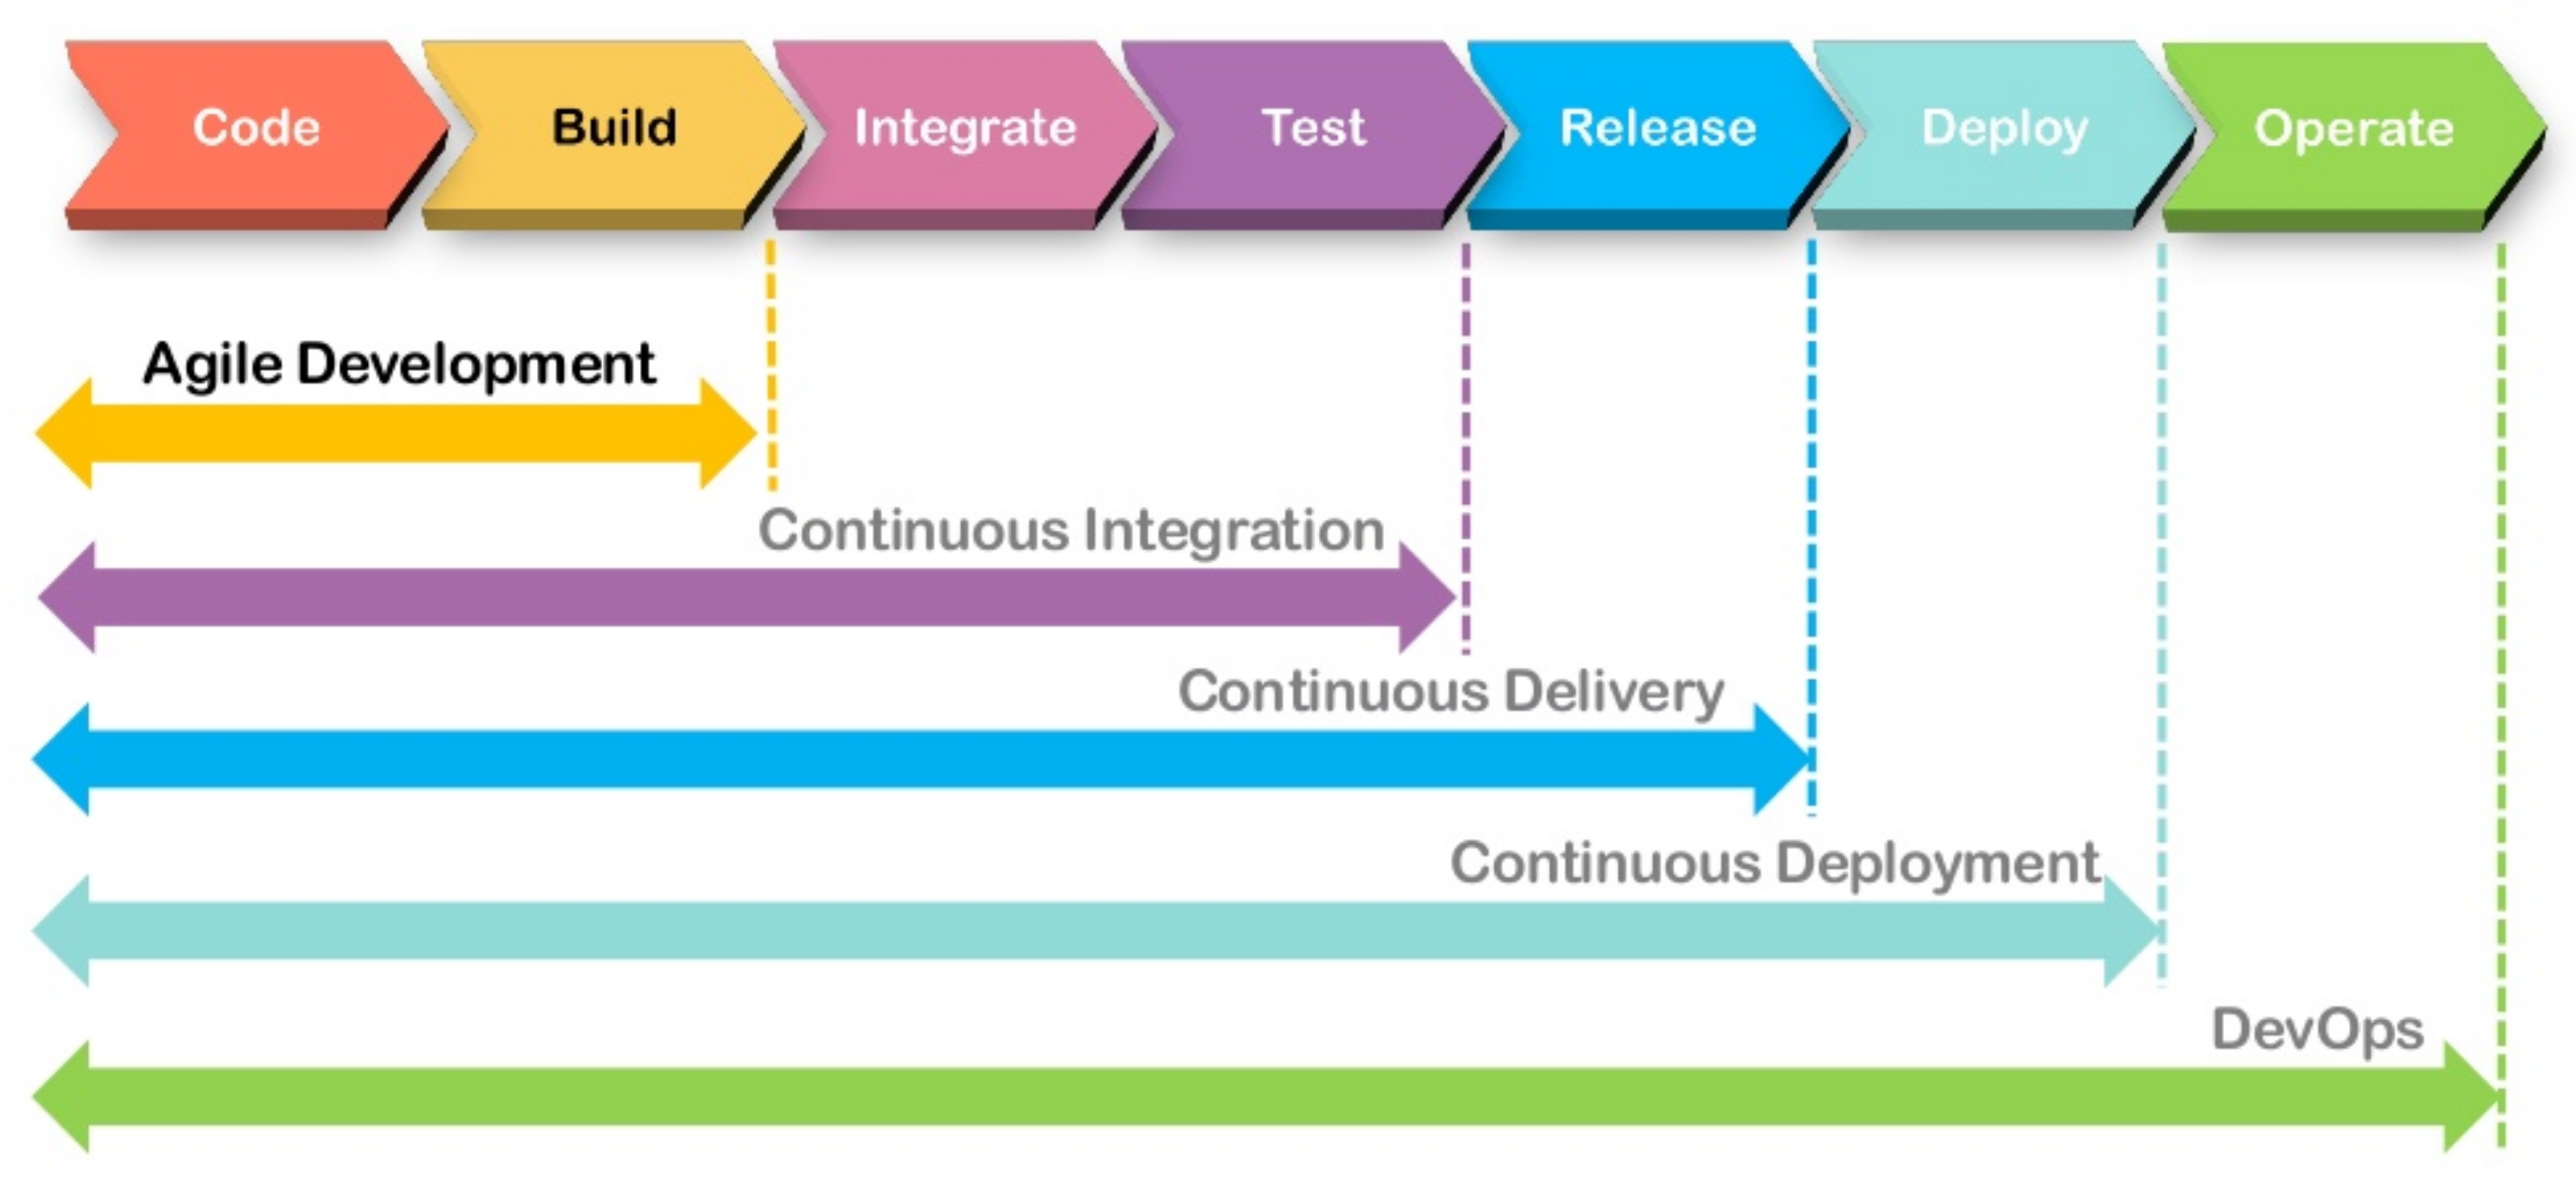
\includegraphics[width=\linewidth]{Images/etapa1}
	\label{fig:etapa1}
\end{figure}
\end{frame}

\begin{frame}{Delivery vs Deployment}
\begin{figure}
	\centering
	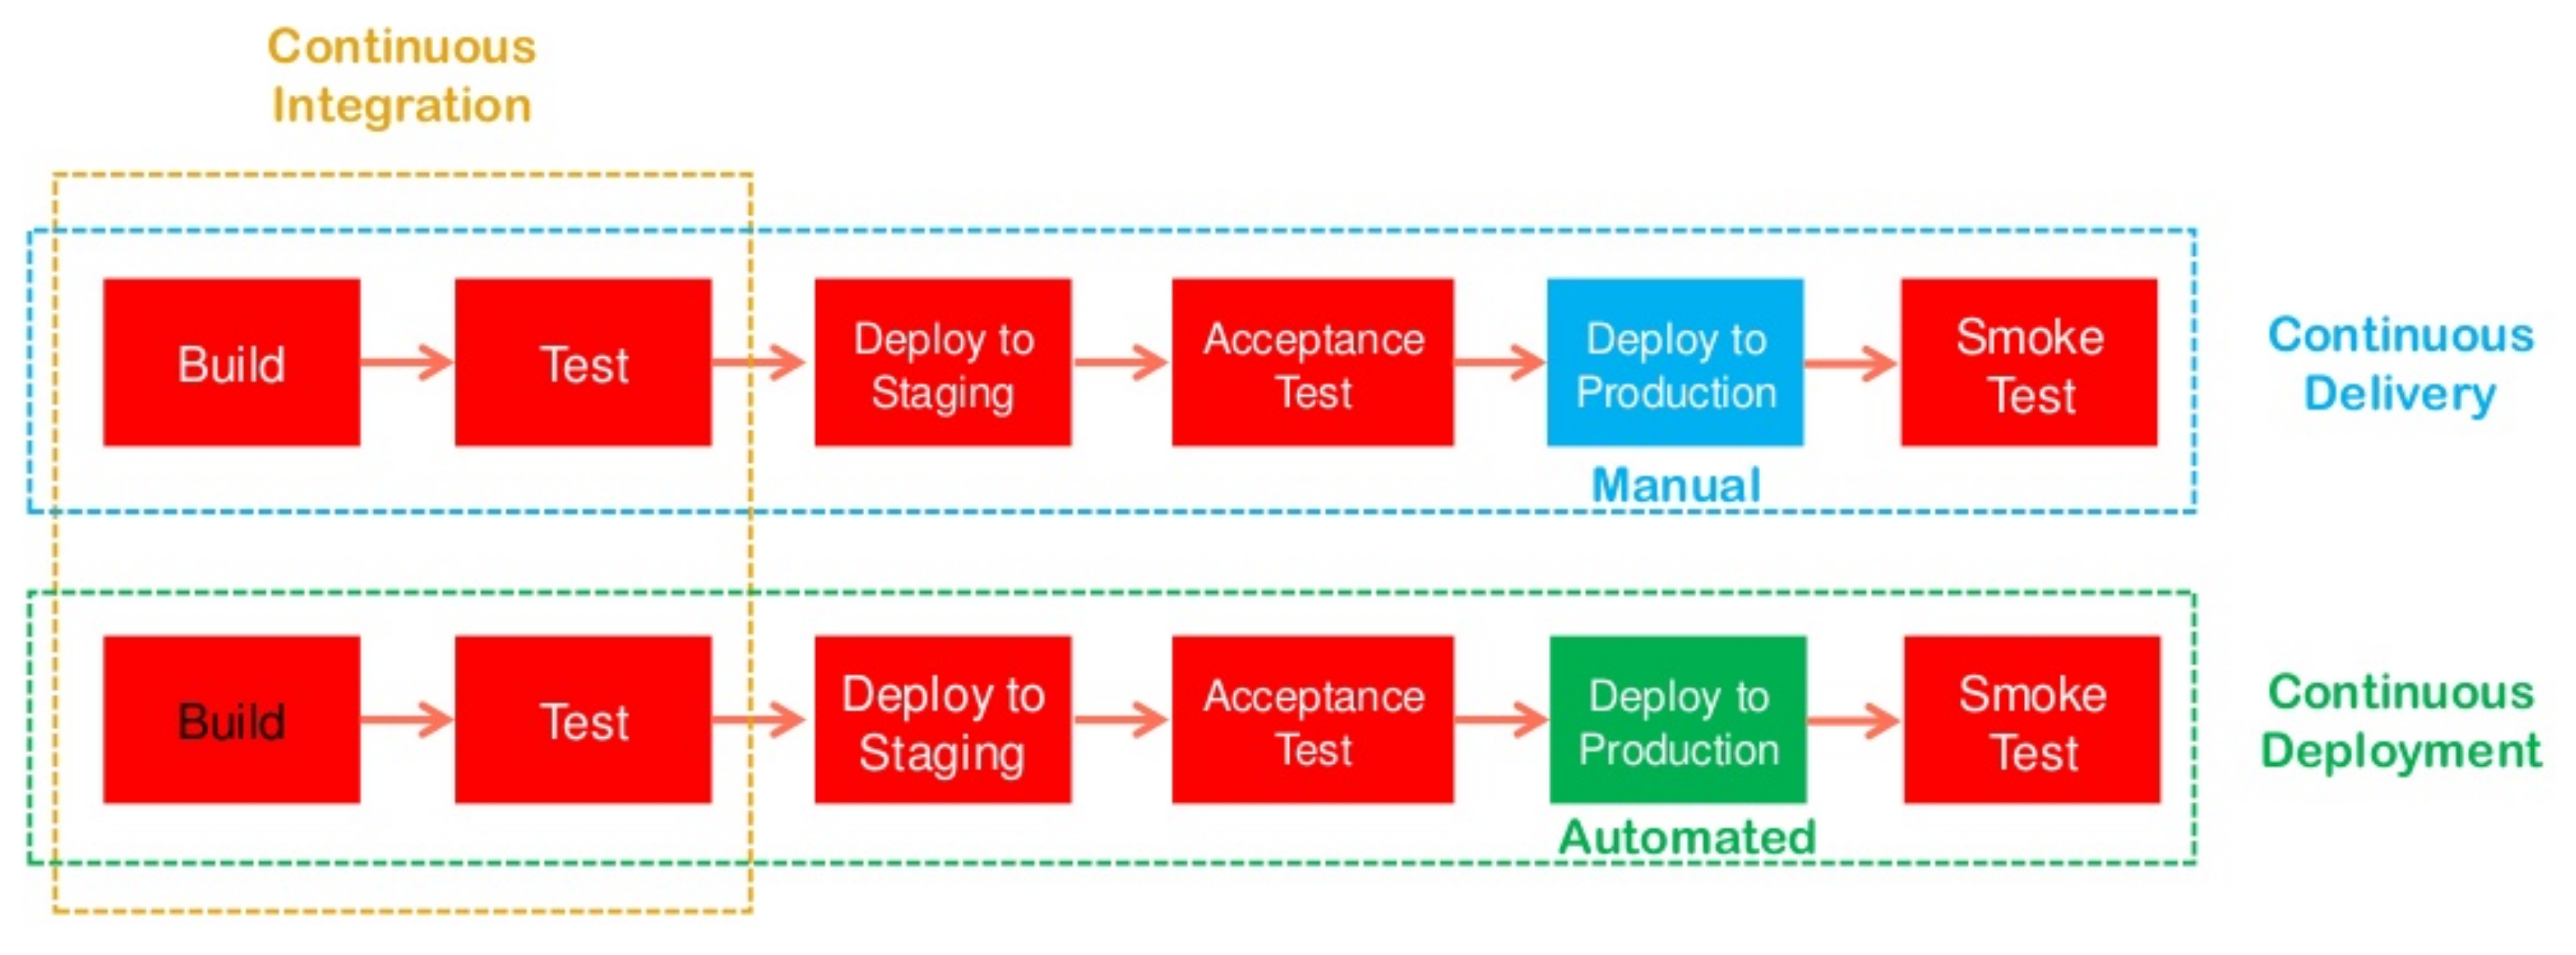
\includegraphics[width=\linewidth]{Images/etapa2}
	\label{fig:etapa2}
\end{figure}
\end{frame}

\begin{frame}{Advertencias}

\begin{alertblock}{Estado del arte en testing}
	El \textit{mundo del testing} es uno de los mundos donde más opiniones existen. Es 100\% seguro que encuentren material que contradiga a este material.
\end{alertblock}

\begin{alertblock}{Disciplinas de testing}
Una de las áreas más subjetivas del software -e.g. CMMI, ISO/IEC 12207, Six Sigma-
\end{alertblock}

\end{frame}


\begin{frame}{Calidad del software}
\begin{figure}
	\centering
	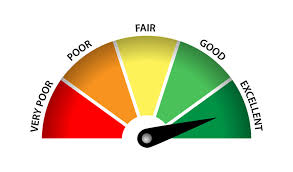
\includegraphics[width=0.6\linewidth]{Images/quality}
\end{figure}
¿Que es?
\end{frame}


\begin{frame}{Calidad del software}
\begin{figure}
	\centering
	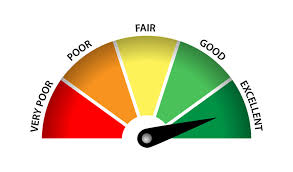
\includegraphics[width=0.6\linewidth]{Images/quality}
\end{figure}
Requerimientos vs. expectativas vs. realidad
\end{frame}

\begin{frame}{Calidad del software}
\begin{columns}[T]
	\begin{column}[T]{5cm}
		\begin{itemize}
			\item \textbf{Calidad:} El grado en el que un componente, sistema o proceso cumple con requerimientos, necesidades y expectativas
			\item \textbf{Calidad en Software:} Funcionalidad y características que hacen que un producto de software satisfagan las necesidades.
		\end{itemize}
	\end{column}
	\begin{column}[T]{5cm} % alternative top-align that's better for graphics
		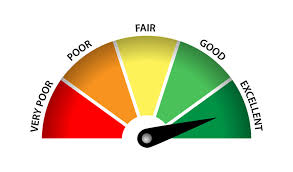
\includegraphics[height=3cm]{Images/quality}
	\end{column}
\end{columns}
\end{frame}

\begin{frame}{Dimensiones}


\begin{block}{Falsa afirmación}
El software es de gran calidad
\end{block}

\pause
¿En que dimensión?
\end{frame}

\begin{frame}{Dimensiones}
\begin{columns}[T]
	\begin{column}[T]{5cm}
		\begin{itemize}
			\item Accesibilidad
			\item Compatibilidad
			\item \textbf{Concurrencia}
			\item \textbf{Eficiencia}
			\item \textbf{Funcionalidad}
			\item Instalabilidad
			\item Localizabilidad
			\item \textbf{Facilidad de mantenimiento}
		\end{itemize}
	\end{column}
	\begin{column}[T]{5cm} % alternative top-align that's better for graphics
		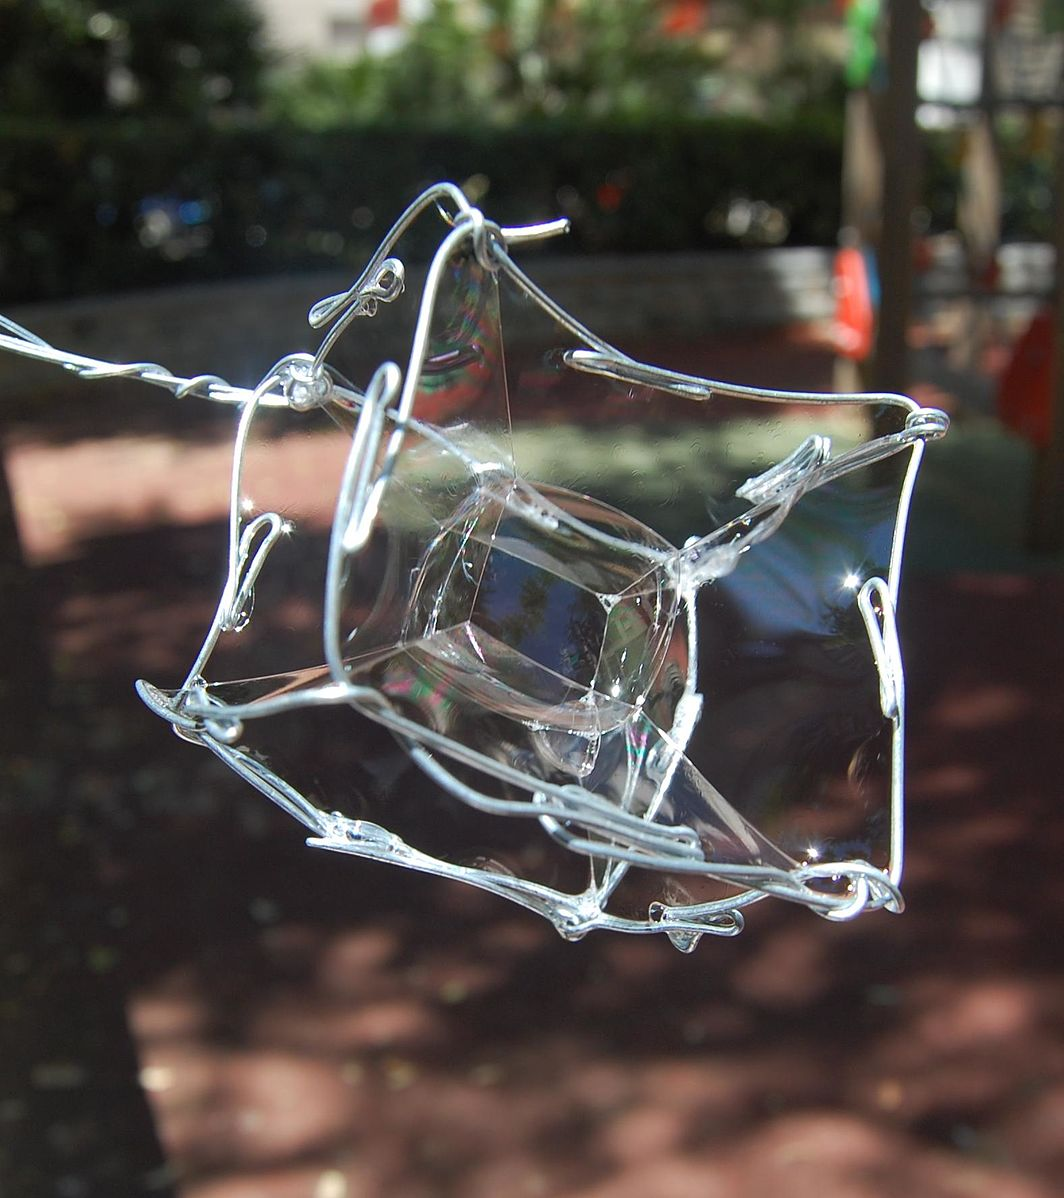
\includegraphics[width=\linewidth]{Images/teseracto}
	\end{column}
\end{columns}
\end{frame}

\begin{frame}{Dimensiones}
\begin{columns}[T]
	\begin{column}[T]{5cm}
		\begin{itemize}
			\item \textbf{Desempeño}
			\item \textbf{Portabilidad}
			\item \textbf{Confiabilidad}
			\item Escalabilidad
			\item \textbf{Seguridad}
			\item Usabilidad
			\item Facilidad de pruebas
		\end{itemize}
	\end{column}
	\begin{column}[T]{5cm} % alternative top-align that's better for graphics
		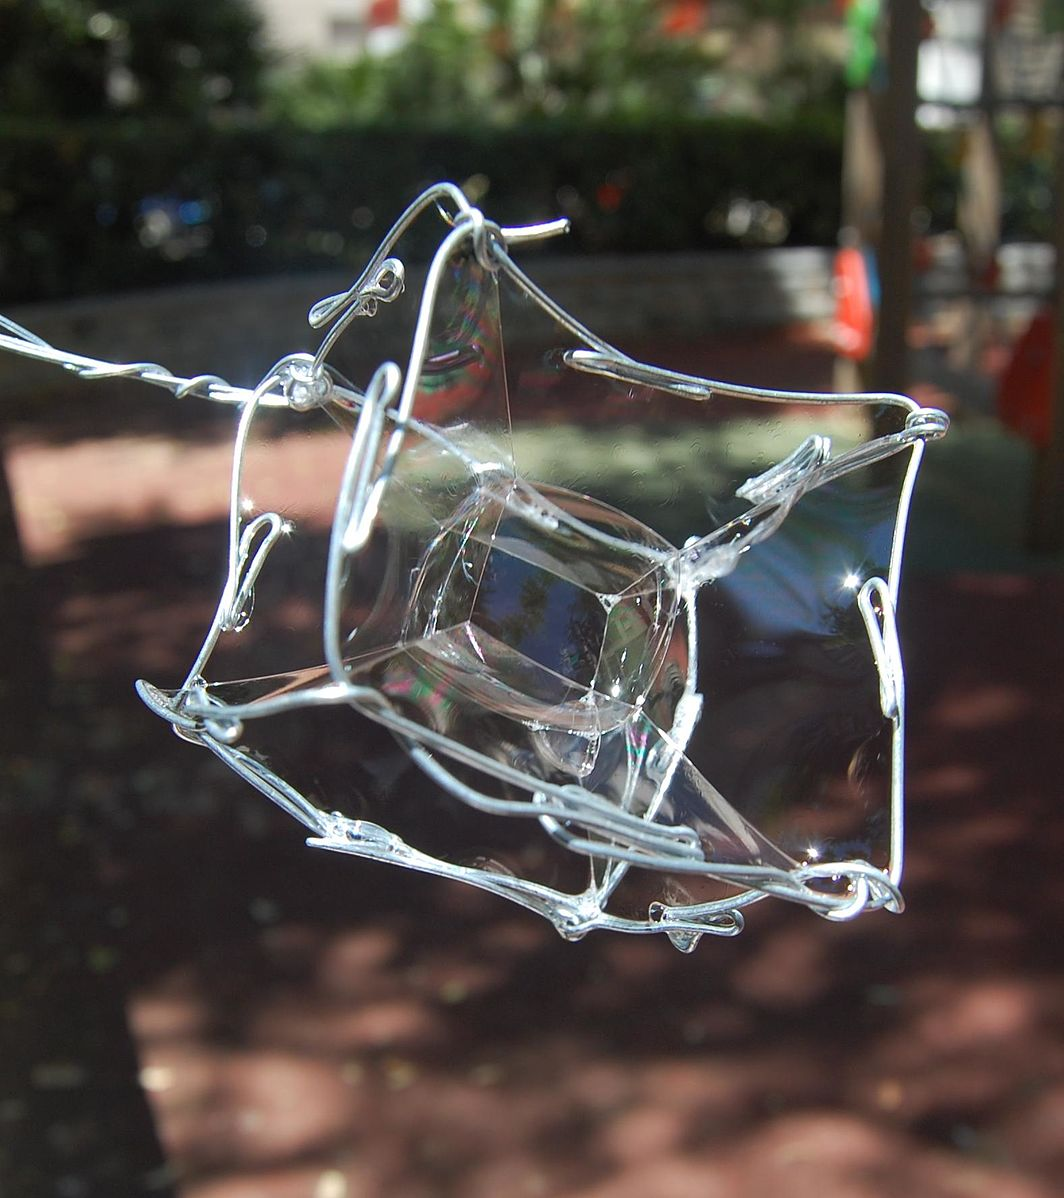
\includegraphics[width=\linewidth]{Images/teseracto}
	\end{column}
\end{columns}
\end{frame}
{
    \usebackgroundtemplate{
\includegraphics[width=\paperwidth]{Images/separador}}
    \setbeamercolor{normal text}{fg=white}
    \setbeamercolor{frametitle}{fg=red}
    \usebeamercolor[fg]{normal text}
\section{SQA y SQC}
}

\begin{frame}{SQA}
\begin{columns}[T]
	\begin{column}[T]{5cm}
		\begin{itemize}
			\item Procesos
			\item Auditoria
			\item Entrenamiento
		\end{itemize}
	¿Cuales procesos?
	\pause
	\end{column}
	\begin{column}[T]{5cm} % alternative top-align that's better for graphics
		\begin{itemize}
			\item Metodología de software
			\item Gestión de proyecto
			\item Administración de la configuración
			\item Requerimientos
			\item Estimaciones
			\item Arquitectura de software
			\item \textbf{Pruebas}
		\end{itemize}
	\end{column}
\end{columns}
\end{frame}

\begin{frame}{SQC}
Objetivo: Que el software cumpla con los requerimientos
\begin{columns}[T]
	\begin{column}[T]{5cm}
		Revisiones
		\begin{itemize}
			\item Requerimientos
			\item Diseño
			\item Código
			\item Plan de despliegue
			\item Plan de testing
			\item Casos de prueba
		\end{itemize}
	\end{column}
	\begin{column}[T]{5cm} % alternative top-align that's better for graphics
		Pruebas
		\begin{itemize}
			\item Unit testing
			\item Integration testing
			\item System testing
			\item Acceptance testing
		\end{itemize}
	Entre otros . . .
	\end{column}
\end{columns}
\end{frame}


\begin{frame}{SQA vs. SQC}
\small
\begin{table}
\begin{tabular}{|c|c|c|}
	\hline 
	Criterio &  SQA &  SQC\\ 
	\hline 
	Definición &  Calidad en el proceso & Calidad en el producto \\ 
	\hline 
	Enfoque & Procesos &  Producto \\ 
	\hline 
	Orientación & Prevención & Detección \\ 
	\hline 
	Alcance & Organizacional  & Por producto/proyecto  \\ 
	\hline 
	Actividades& Procesos, auditoria y entrenamiento & Revisiones y pruebas \\ 
	\hline 
\end{tabular} 
\end{table} 
\end{frame}


{
    \usebackgroundtemplate{
\includegraphics[width=\paperwidth]{Images/separador}}
    \setbeamercolor{normal text}{fg=white}
    \setbeamercolor{frametitle}{fg=red}
    \usebeamercolor[fg]{normal text}
    \section{SQC}
    }

\begin{frame}{Pruebas}
\begin{figure}
	\centering
	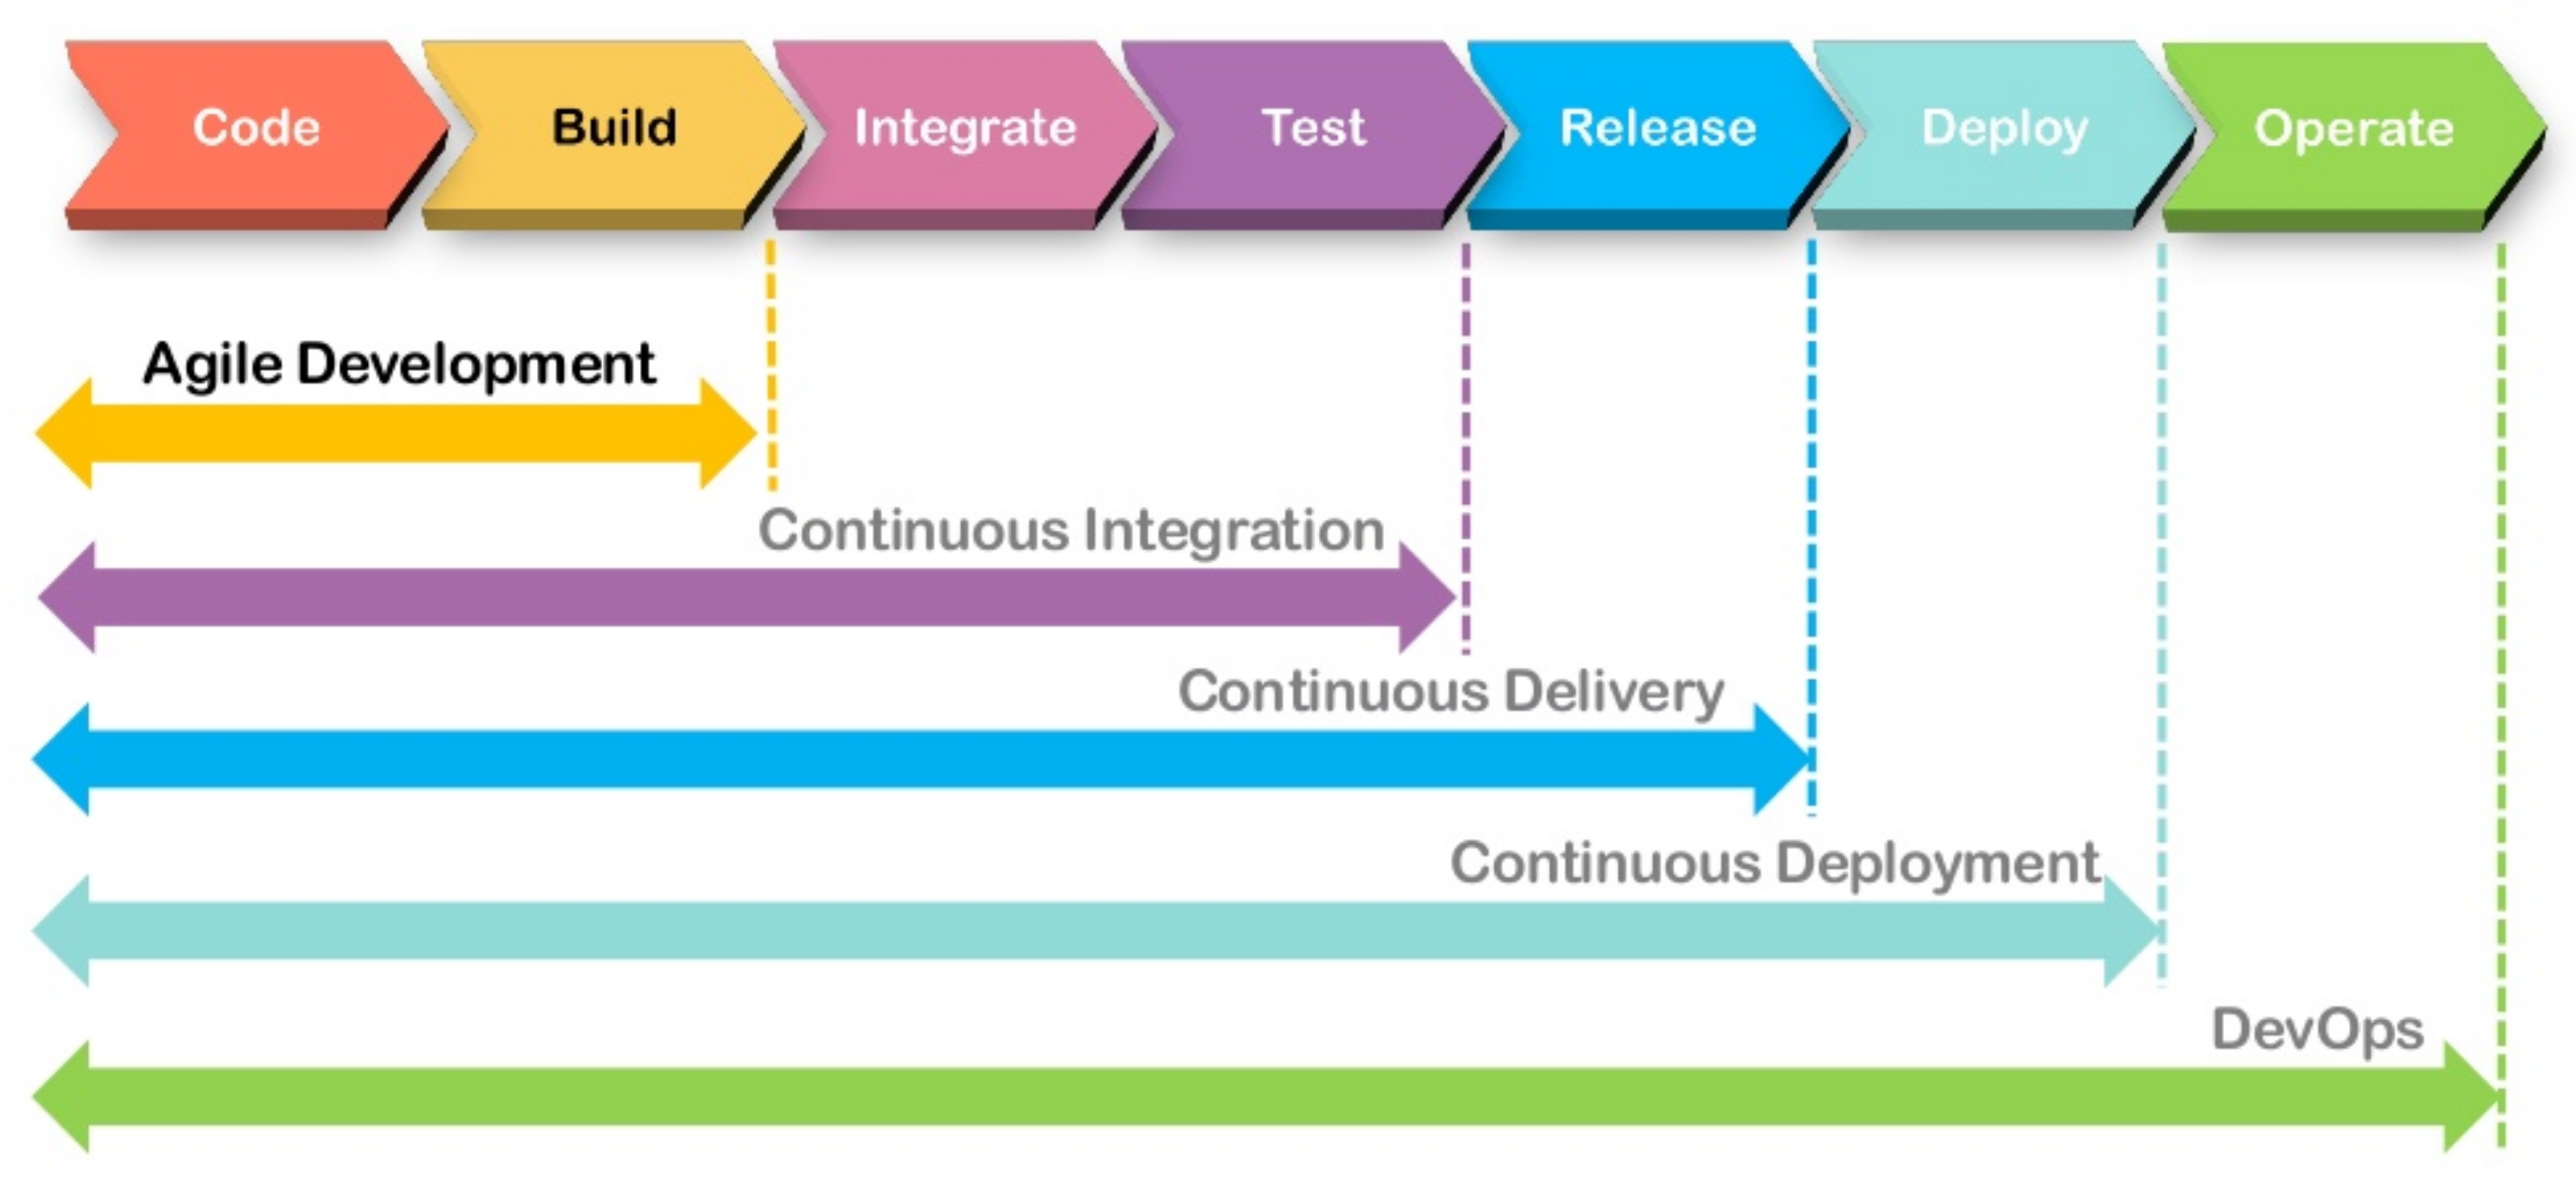
\includegraphics[width=\linewidth]{Images/etapa1}
\end{figure}
\end{frame}

\begin{frame}{Pruebas}
\begin{columns}[T]
	\begin{column}[T]{5cm}
		Preparación (revisión)
		\begin{itemize}
			\item Requerimientos
			\item Diseño
			\item Código
			\item Plan de despliegue
			\item Plan de pruebas
			\item Casos de prueba
		\end{itemize}
	\end{column}
	\begin{column}[T]{5cm} % alternative top-align that's better for graphics
		Pruebas
		\begin{itemize}
			\item Unit testing
			\item Integration testing
			\item System testing
			\item Acceptance testing
		\end{itemize}
	\end{column}
\end{columns}
\end{frame}

\begin{frame}{Pruebas}
\begin{figure}
	\centering
	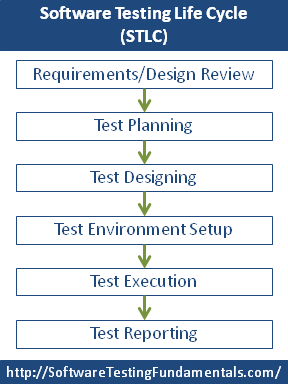
\includegraphics[width=0.4\linewidth]{Images/lifecycle}
\end{figure}
\end{frame}


\begin{frame}{Unit Testing - Tipos}
\begin{columns}[T]
	\begin{column}[T]{6cm}
		\begin{itemize}
			\item Funcionamiento de cada unidad
			\item Estructurado: Programa, función, procedimiento
			\item POO: Clase y derivados (servicio, endpoint)
			\item Frameworks, drivers, stubs, mocks
			\item Developers
			\item Tip: Probar lo que tiene impacto
		\end{itemize}
	\end{column}
	\begin{column}[T]{4cm} % alternative top-align that's better for graphics
\begin{figure}
	\centering
	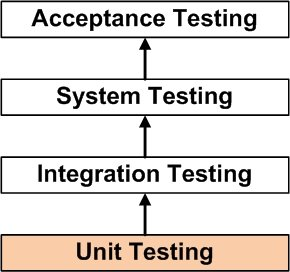
\includegraphics[width=0.8\linewidth]{Images/unittesting}
\end{figure}
	\end{column}
\end{columns}
\end{frame}

\begin{frame}{Integration Testing - Tipos}
\begin{columns}[T]
	\begin{column}[T]{6cm}
		\begin{itemize}
			\item Unidades combinadas
			\item Interfaces e integraciones
			\item Sistemas externos
			\item Frameworks, White Box, Black Box
			\item Developers y testers
			\item Tip: Documentar integraciones
		\end{itemize}
	\end{column}
	\begin{column}[T]{4cm} % alternative top-align that's better for graphics
		\begin{figure}
			\centering
			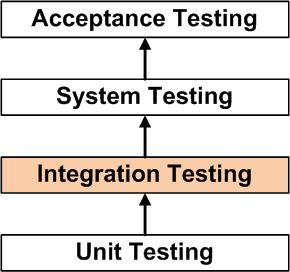
\includegraphics[width=0.8\linewidth]{Images/integrationtesting}
		\end{figure}
	\end{column}
\end{columns}
\end{frame}

\begin{frame}{System Testing - Tipos}
\begin{columns}[T]
	\begin{column}[T]{6cm}
		\begin{itemize}
			\item Sistema vs. requerimientos
			\item Black Box
			\item Testers
			\item Tip: Requerimientos actualizados
		\end{itemize}
	\end{column}
	\begin{column}[T]{4cm} % alternative top-align that's better for graphics
		\begin{figure}
			\centering
			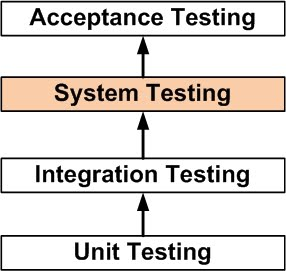
\includegraphics[width=0.8\linewidth]{Images/systemtesting}
		\end{figure}
	\end{column}
\end{columns}
\end{frame}

\begin{frame}{Acceptance Testing - Tipos}
\begin{columns}[T]
	\begin{column}[T]{6cm}
		\begin{itemize}
			\item Requerimientos vs. necesidades reales
			\item Ad-hoc
			\item Pruebas internas: Alpha, Testers
			\item Pruebas externas: Beta, Usuarios y clientes
		\end{itemize}
	\end{column}
	\begin{column}[T]{4cm} % alternative top-align that's better for graphics
		\begin{figure}
			\centering
			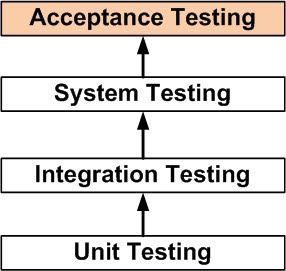
\includegraphics[width=0.8\linewidth]{Images/acceptancetesting}
		\end{figure}
	\end{column}
\end{columns}
\end{frame}


\begin{frame}{Black box - Técnicas}
\begin{columns}[T]
	\begin{column}[T]{4cm}
		\begin{itemize}
			\item Integration
			\item System
			\item Acceptance
		\end{itemize}
	\end{column}
	\begin{column}[T]{6cm} % alternative top-align that's better for graphics
		\begin{figure}
			\centering
			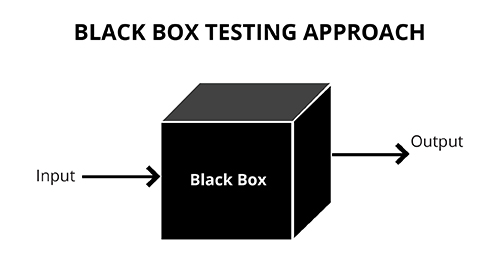
\includegraphics[width=\linewidth]{Images/blackboxtesting.jpg}
		\end{figure}
	\end{column}
\end{columns}
\end{frame}

\begin{frame}{White box - Técnicas}
\begin{columns}[T]
	\begin{column}[T]{4cm}
		\begin{itemize}
			\item Unit
			\item Integration
			\item System

		\end{itemize}
	\end{column}
	\begin{column}[T]{6cm} % alternative top-align that's better for graphics
		\begin{figure}
			\centering
			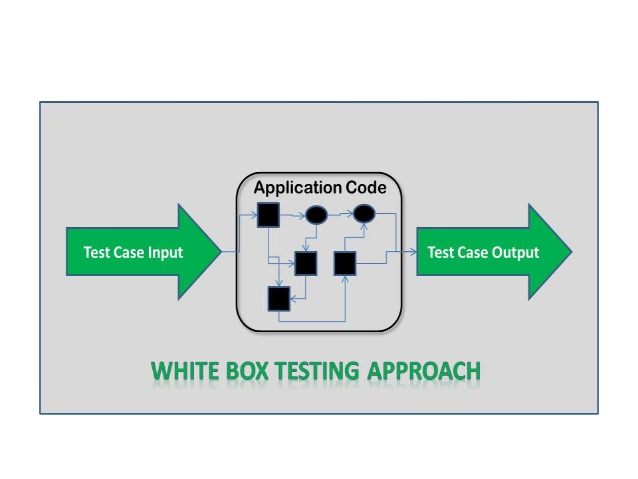
\includegraphics[width=\linewidth]{Images/whiteboxtesting.jpg}
		\end{figure}
	\end{column}
\end{columns}
\end{frame}


\begin{frame}{Ad hoc - Técnicas}
\begin{columns}[T]
	\begin{column}[T]{4cm}
		\begin{itemize}
			\item Acceptance
			\item Monkey Testing
		\end{itemize}
	\end{column}
	\begin{column}[T]{6cm} % alternative top-align that's better for graphics
		\begin{figure}
			\centering
			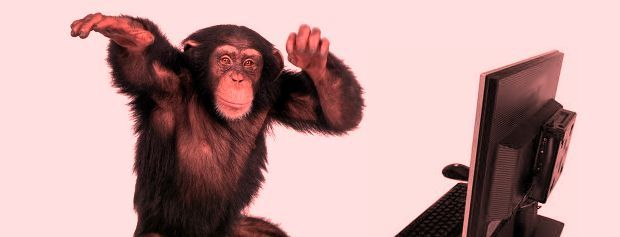
\includegraphics[width=\linewidth]{Images/adhoctesting.jpg}
		\end{figure}
	\end{column}
\end{columns}
\end{frame}


\begin{frame}{TDD - Técnicas}
\begin{columns}[T]
	\begin{column}[T]{4cm}
		\begin{itemize}
			\item Unit
			\item Integration
		\end{itemize}
	\end{column}
	\begin{column}[T]{6cm} % alternative top-align that's better for graphics
		\begin{figure}
			\centering
			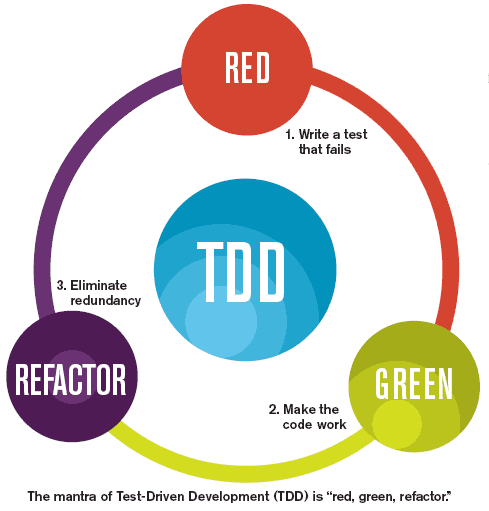
\includegraphics[width=0.9\linewidth]{Images/tdd}
		\end{figure}
	\end{column}
\end{columns}
\end{frame}


\begin{frame}{Gracias}
\begin{itemize}
\item vorozco@nabenik.com
\item http://nabenik.com
\end{itemize}
\begin{center}

\includegraphics[width=0.1\linewidth]{Images/cclogo}
\\
This work is licensed under a Creative Commons Attribution-ShareAlike 3.0 Guatemala License.
\end{center}
\end{frame}
\end{document}

